% Convert with command:
% convert -density 300 pic.pdf -quality 90 pic.png
\documentclass[crop,tikz,border=0pt]{standalone}
\usetikzlibrary{arrows.meta}
\begin{document}
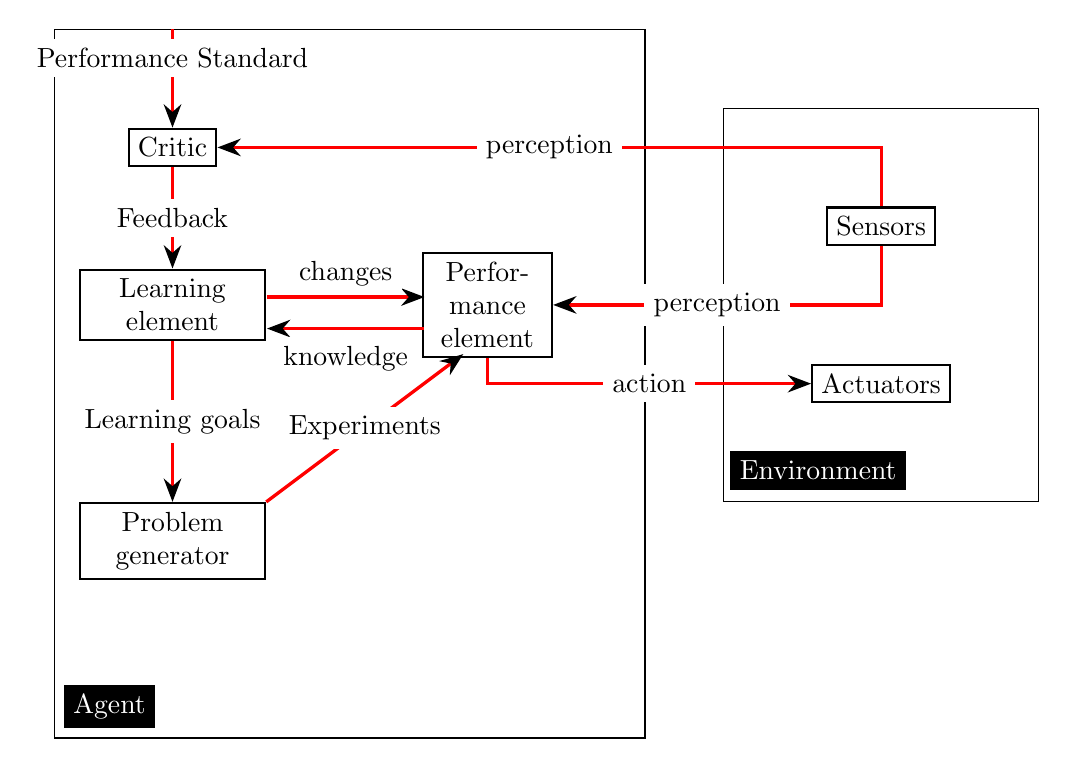
\begin{tikzpicture}

\begin{scope}[every node/.style={circle,thick,draw,fill=white}]
    % Scene rectangles
    \draw (-2.5,0) rectangle (5,9) [fill=white] {};
    \draw (6,3) rectangle (10,8) [fill=white] {};

    \node (A) at (3,5.5) [shape=rectangle, text width=4em, text centered] 
        {Perfor-mance element};

    \node (B) at (-1, 7.5) [shape=rectangle] 
        {Critic};

    \node (C) at (-1,5.5) [shape=rectangle, text width=6em, text centered] 
        {Learning element};

    \node (D) at (-1,2.5) [shape=rectangle, text width=6em, text centered] 
        {Problem generator};

    % Right rectangle - environment
    \node (G) at (8,6.5)[shape=rectangle, fill=white] {Sensors};
    \node (H) at (8,4.5)[shape=rectangle, fill=white] {Actuators};
\end{scope}

\tikzset{CustomEdge/.style={fill=white,rectangle,text=black}}

\begin{scope}[>={Stealth[black]},
            %   every node/.style={fill=white,rectangle},
            %   every node/.style={},
              every edge/.style={draw=red,very thick}]
    \draw [->, red, very thick] (G) |- node [CustomEdge, near end] {perception} (A);
    \draw [->, red, very thick] (G) |- node [CustomEdge, near end] {perception} (B);
    \path [->] (-1, 9) edge [] node [CustomEdge, above] {Performance Standard} (B);

    \path [->] (B) edge node [CustomEdge] {Feedback} (C);

    \path [->] (C) edge node [CustomEdge] {Learning goals} (D);

    \path [->] (0.2, 5.6) edge node [CustomEdge, above] {changes} (2.2, 5.6);

    \path [<-] (0.2, 5.2) edge node [CustomEdge, below, yshift=-0.25em] {knowledge} (2.2, 5.2);

    \path [->] (D) edge [transform canvas={xshift=1.5em}] node [CustomEdge] {Experiments} (A);

    \draw [->, red, very thick] (A) |- node [CustomEdge, near end] {action} (H);
\end{scope}

% \draw (0,1) node [] {Text at \verb!node A!};

\draw (-1.8,0.4) node [rectangle, draw, fill=black, text=white] {Agent};

\draw (7.2,3.4) node [rectangle, draw, fill=black, text=white] {Environment};

\end{tikzpicture}
\end{document}
